% !TeX root = ../paper.tex


\section{Symmetric Entropic Affinities}\label{sec:sym_entropic_affinity}

In this section, we present our first major contribution: symmetric entropic affinities. We begin by providing a new perspective on EAs through the introduction of an equivalent convex problem.

\subsection{Entropic Affinities as Entropic Optimal Transport}\label{sec:entropic_affinity_semi_relaxed}

We introduce the following set of matrices with row-wise stochasticity and entropy constraints:
\begin{align}
  \mathcal{H}_\xi = \{\Pb \in \mathbb{R}_+^{n \times n} \ \text{s.t.} \ \Pb \bm{1} = \bm{1} \: \ \text{and} \  \forall i, \: \operatorname{H}(\Pb_{i:}) \geq \log{\xi} + 1 \}\:.
\end{align}
This space is convex since $\mathbf{p} \in \R_+^n \mapsto \operatorname{H}(\mathbf{p})$ is concave, thus its superlevel set is convex. In contrast to the entropic constraints utilized in standard entropic optimal transport which set a lower-bound on the \emph{global} entropy, as demonstrated in the formulation \eqref{eq:entropy_constrained_OT}, $\mathcal{H}_\xi$ imposes a constraint on the entropy of \emph{each row} of the matrix $\Pb$.
Our first contribution is to prove that EAs can be computed by solving a specific problem involving $\mathcal{H}_\xi$ (see Appendix \ref{sec:proofs} for the proof).
\begin{restatable}{proposition}{entropicaffinityaslinearprogram}
\label{prop:entropic_affinity_as_linear_program}
Let $\Cb \in \R^{n \times n}$ without constant rows. Then $\Pb^{\mathrm{e}}$ solves the entropic affinity problem (\ref{eq:entropic_affinity_pb}) with cost $\Cb$ if and only if $\Pb^{\mathrm{e}}$ is the unique solution of the convex problem
\begin{equation}\label{eq:entropic_affinity_semi_relaxed}
    \min_{\Pb \in \mathcal{H}_{\xi}} \: \langle \Pb, \Cb \rangle .
    \tag{EA as OT}
\end{equation}
\end{restatable}
Interestingly, this result shows that EAs boil down to minimizing a transport objective with cost $\Cb$ and row-wise entropy constraints $\mathcal{H}_{\xi}$ where
$\xi$ is the desired perplexity. As such, \eqref{eq:entropic_affinity_semi_relaxed} can be seen as a specific \emph{semi-relaxed} OT problem \citep{rabin2014adaptive,flamary2016optimal} (\ie without the second constraint on the marginal $\Pb^\top \bm{1}= \bm{1}$) but with entropic constraints on the rows of $\Pb$. We also show that the optimal solution $\Pb^\star$ of \eqref{eq:entropic_affinity_semi_relaxed} has \emph{saturated entropy} \ie $\forall i, \: \operatorname{H}(\Pb^\star_{i:}) = \log{\xi} + 1$. In other words, relaxing the equality constraint in \eqref{eq:entropic_affinity_pb} as a inequality constraint in $\Pb \in \mathcal{H}_{\xi}$ does not affect the solution while it allows reformulating entropic affinity as a convex optimization problem. To the best of our knowledge, this connection between OT and entropic affinities is novel and is an essential key to the method proposed in the
next section.
% To gain intuition on the entropy saturation at the optimum, one can simply notice that, since $\Cb \in
% \mathcal{D}$, transferring some mass from anywhere off-diagonal to the diagonal
% decreases both the objective and the entropy.

\begin{remark}
  The kernel bandwidth parameter $\bm{\varepsilon}$ from the original formulation of entropic affinities (\ref{eq:entropic_affinity_pb}) is the Lagrange dual variable associated with the entropy constraint in (\ref{eq:entropic_affinity_semi_relaxed}). Hence computing $\bm{\varepsilon}^\star$ in (\ref{eq:entropic_affinity_pb}) exactly corresponds to solving the dual problem of (\ref{eq:entropic_affinity_semi_relaxed}).
\end{remark}

\begin{remark}\label{Pe_proj}
  Let $\K_{\sigma} = \exp(-\Cb / \sigma)$. As shown in \cref{sec:proj_KL}, if $\bm{\varepsilon}^\star$ solves (\ref{eq:entropic_affinity_pb}) and $\sigma \leq \min(\bm{\varepsilon}^\star)$, then $\Pb^{\mathrm{e}} = \operatorname{Proj}^{\operatorname{\KL}}_{\mathcal{H}_{\xi}}(\K_{\sigma})  =  \argmin_{\Pb \in \mathcal{H}_{\xi}} \KL(\Pb | \K_\sigma)$.
  Therefore $\Pb^{\mathrm{e}}$ can be seen as a $\KL$ Bregman projection \citep{benamou2015iterative} of a Gaussian kernel onto $\mathcal{H}_{\xi}$. Hence the input matrix in \eqref{symmetrization_tsne}  is $\overline{\Pb^{\mathrm{e}}}= \operatorname{Proj}^{\ell_2}_{\mathcal{S}}(\operatorname{Proj}^{\operatorname{\KL}}_{\mathcal{H}_{\xi}}(\K_\sigma))$ which corresponds to a surprising mixture of $\KL$ and orthogonal projections.
\end{remark}

\subsection{Symmetric Entropic Affinity Formulation}\label{subsec:sea}

\begin{figure*}[t]
  \begin{center}
  \centerline{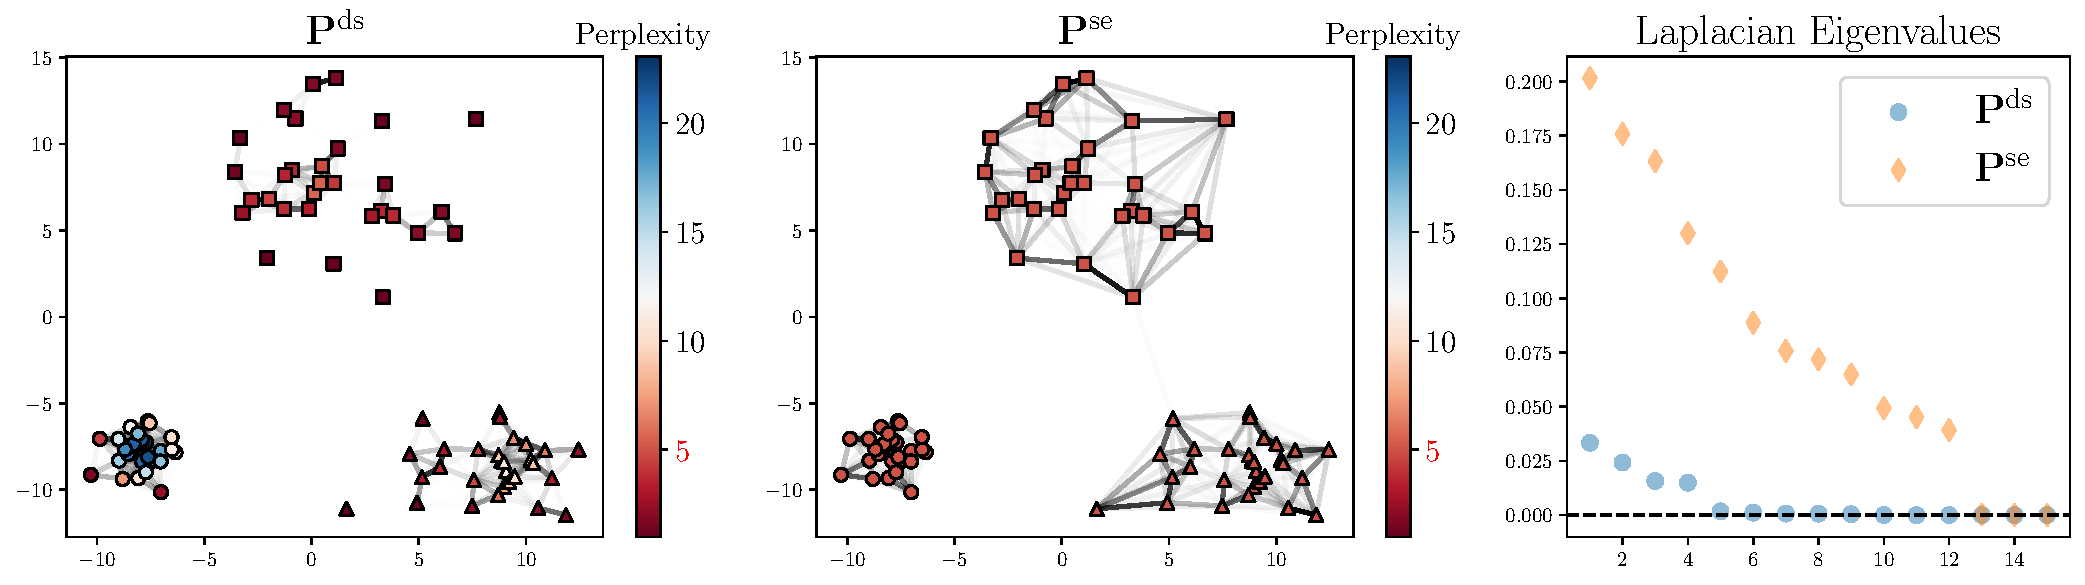
\includegraphics[width=\columnwidth]{figures/SNEkhorn/Ps_vs_Pse.pdf}}
  \caption{Samples from a mixture of three Gaussians with varying standard deviations. The edges' strength is proportional to the weights in the affinities $\Pb^{\mathrm{ds}}$ \eqref{eq:plan_sym_sinkhorn} and $\Pb^{\mathrm{se}}$ \eqref{eq:sym_entropic_affinity} computed with $\xi=5$ (for $\Pb^{\mathrm{ds}}$, $\xi$ is the average perplexity such that $\sum_i \operatorname{H}(\Pb^{\mathrm{ds}}_{i:})=\sum_i \operatorname{H}(\Pb^{\mathrm{se}}_{i:})$). Points' color represents the perplexity $e^{\operatorname{H}(\Pb_{i:})-1}$. Right plot: smallest eigenvalues of the Laplacian for the two affinities.}
  \label{fig:Ps_vs_Pse}
  \end{center}
\end{figure*}

Based on the previous formulation we now propose symmetric entropic affinities: a symmetric version of EAs that enables keeping the entropy associated with each row (or equivalently column) to the desired value of $\log \xi + 1$ while producing a symmetric doubly stochastic affinity matrix. Our strategy is to enforce symmetry through an additional constraint in (\ref{eq:entropic_affinity_semi_relaxed}), in a similar fashion as \eqref{eq:entropy_constrained_OT}. More precisely we consider the convex optimization problem
\begin{align}
\label{eq:sym_entropic_affinity}
\tag{SEA}
  \min_{\Pb \in \mathcal{H}_{\xi} \cap \mathcal{S}} \: \langle \Pb, \Cb \rangle \:. 
\end{align}
where we recall that $\mathcal{S}$ is the set of $n \times n$ symmetric matrices. Note that for any $\xi \leq n-1$, $\frac{1}{n} \bm{1}\bm{1}^\top \in \mathcal{H}_{\xi} \cap \mathcal{S}$ hence the set $\mathcal{H}_{\xi} \cap \mathcal{S}$ is a non-empty and convex set. We first detail some important properties of problem \eqref{eq:sym_entropic_affinity} (the proofs of the following results can be found in Appendix \ref{proof:main_props}).
\begin{restatable}[Saturation of the entropies]{proposition}{saturation}
\label{prop:saturation_entropies}
Let $\Cb \in \mathcal{S}$ with zero diagonal, then \eqref{eq:sym_entropic_affinity} with cost $\Cb$ has a \emph{unique solution} that we denote by $\Pb^{\mathrm{se}}$. If moreover $\Cb \in \mathcal{D}$, then for at least $n-1$ indices $i \in \integ{n}$ the solution satisfies $\operatorname{H}(\Pb^{\mathrm{se}}_{i:}) = \log \xi + 1$.
\end{restatable}
In other words, the unique solution $\Pb^{\mathrm{se}}$ has at least $n-1$ saturated entropies \ie the corresponding $n-1$ points have exactly a perplexity of $\xi$. In practice, with the algorithmic solution detailed below, we have observed that all $n$ entropies are saturated. Therefore, we believe that this proposition can be extended with a few more assumptions on $\Cb$. Accordingly,
problem \Cref{eq:sym_entropic_affinity} allows accurate control over the point-wise entropies while providing a symmetric doubly stochastic matrix, unlike $\overline{\Pb^{\mathrm{e}}}$ defined in
\Cref{sec:background_dr}, as summarized in \Cref{fig:recap_properties_sym}. In the sequel, we denote by $\operatorname{H}_{\mathrm{r}}(\Pb) = \left( \operatorname{H}(\Pb_{i:}) \right)_{i}$ the vector of row-wise entropies of $\Pb$. We rely on the following result to compute $\Pb^{\mathrm{se}}$.
\begin{restatable}[Solving for \ref{eq:sym_entropic_affinity}]{proposition}{solvingsea}
\label{prop:sol_gamma_non_null}
Let $\Cb \in \mathcal{D}, \mathcal{L}(\Pb, \bm{\gamma}, \bm{\lambda})= \langle \Pb, \Cb \rangle + \langle \gammab, (\log{\xi} + 1) \bm{1} - \operatorname{H}_{\mathrm{r}}(\Pb) \rangle + \langle \lambdab, \bm{1} - \Pb \bm{1} \rangle$ and $q(\bm{\gamma}, \bm{\lambda}) = \min_{\Pb \in \R_{+}^{n \times n} \cap \mathcal{S}} \mathcal{L}(\Pb, \bm{\gamma}, \bm{\lambda})$. Strong duality holds for \eqref{eq:sym_entropic_affinity}. Moreover, let
$\bm{\gamma}^\star, \lambdab^\star \in \operatorname{argmax}_{\bm{\gamma} \geq 0, \lambdab} q(\bm{\gamma}, \bm{\lambda})$ be the optimal dual variables respectively associated with the entropy and marginal constraints. Then, for at least $n-1$ indices $i \in \integ{n}, \gamma^{\star}_i > 0$.
When $\forall i \in \integ{n}$, $\gamma^\star_i > 0$ then $\operatorname{H}_{\mathrm{r}}(\Pb^{\mathrm{se}}) = (\log \xi + 1)\bm{1}$ and $\Pb^{\mathrm{se}}$ has the form
\begin{align}
    \Pb^{\mathrm{se}} &= \exp{\left(\left(\lambdab^\star \oplus \lambdab^\star - 2 \Cb \right) \oslash \left(\bm{\gamma}^\star \oplus \bm{\gamma}^\star \right) \right)} \:.
   % \label{eq:optimal_P_se}
\end{align}
\end{restatable}
% To set the dual variables to their optimal value, a direct approach consists in solving the following dual problem which is concave, denoting $\Pb^{\star}(\gammab, \lambdab) = \exp{\left(\left(\lambdab \oplus \lambdab - 2 \Cb \right) \oslash \left(\bm{\gamma} \oplus \bm{\gamma} \right) \right)}$.
% \begin{align}\label{eq:dual_problem}\tag{Dual-SEA}
%   \max_{\gammab, \lambdab} \: \min_{\Pb \in \mathcal{S}} \quad \langle \Pb, \Cb \rangle + \langle \gammab, (\log{\xi} + 1) \bm{1} - \operatorname{H}_{\mathrm{r}}(\Pb) \rangle + \langle \lambdab, \bm{1} - \Pb \bm{1} \rangle \:.
% \end{align}
% \begin{align}\label{eq:dual_problem}\tag{Dual-SEA}
%   \max_{\gammab \bm{>} \bm{0}, \lambdab}  \quad \langle \Pb^\star(\gammab, \lambdab), \Cb \rangle + \langle \gammab, (\log{\xi} + 1) \bm{1} - \bm{h}^\star(\gammab, \lambdab) \rangle + \langle \lambdab, \bm{1} - \Pb^\star(\gammab, \lambdab) \bm{1} \rangle
% \end{align}
% \begin{proposition}[Unicity and entropy of the solution]\label{prop:sol_sym_perp}
%   \eqref{eq:sym_entropic_affinity} has a unique solution denoted $\Pb^{\mathrm{se}}$. Moreover, for at least $n-1$ indices $i \in \integ{n}$, it holds $\operatorname{H}(\Pb^{\mathrm{se}}_{i:}) = \log \xi + 1$.
% \end{proposition}
% This has minor impacts on the overall control of the entropies especially when $n$ is large. 
% \hug{faux et on a abandonné:
% Moreover, in appendix \ref{sec:all_entropies_saturated}, we provide a sufficient condition on $\Cb$ for $\operatorname{H}(\Pb^{\mathrm{se}}_{i:}) = \log \xi + 1$ to hold for any $i \in \integ{n}$. We found this condition to be mild in practice.}
% Though we did not manage to prove it rigorously, 
By defining the symmetric matrix $\Pb(\bm{\gamma}, \bm{\lambda}) = 
\exp{\left(\left(\lambdab \oplus \lambdab - 2 \Cb \right) \oslash \left(\bm{\gamma} \oplus \bm{\gamma} \right) \right)}$, we prove that, when $\bm{\gamma}>0, \min_{\Pb \in \mathcal{S}} \mathcal{L}(\Pb, \bm{\gamma}, \bm{\lambda})$ has a unique solution given by $\Pb(\bm{\gamma}, \bm{\lambda})$ which implies $q(\gammab, \lambdab) = \mathcal{L}(\Pb(\bm{\gamma}, \bm{\lambda}), \gammab, \lambdab)$. Thus the proposition shows that when $\bm{\gamma}^\star > 0, \ \Pb^{\mathrm{se}} = \Pb(\bm{\gamma}^\star, \bm{\lambda}^\star)$ where $\bm{\gamma}^\star, \bm{\lambda}^\star$ solve the \emph{concave} dual problem 
\begin{equation}
\label{eq:dual_problem}
\tag{Dual-SEA}
\max_{\bm{\gamma} > 0, \lambdab} \mathcal{L}(\Pb(\bm{\gamma}, \bm{\lambda}), \bm{\gamma}, \bm{\lambda}). 
% \text{ where } \Pb(\bm{\gamma}, \bm{\lambda}) := 
% \exp{\left(\left(\lambdab \oplus \lambdab - 2 \Cb \right) \oslash \left(\bm{\gamma} \oplus \bm{\gamma} \right) \right)}
\end{equation}
% As stated in the above result, one can easily see that our proposed
% symmetrization always provides guarantees over the saturation of $n-1$ entropies
% at the optimum. Indeed, let us imagine that there exists two rows $(\ell,
% \ell')$ for which the entropies are strictly greater than $\log \xi + 1$. 
% \begin{wraptable}[9]{R}{7cm}
%   \caption{Properties of $\Pb^{\mathrm{e}}$, $\overline{\Pb^{\mathrm{e}}}$, $\Pb^{\mathrm{ds}}$ and $\Pb^{\mathrm{se}}$}
%   % \begin{small}
%   %  \begin{minipage}{7cm}
%   \begin{sc} \setlength\tabcolsep{1mm}
%   \begin{tabular}{lcccc}
%   \toprule[1.5pt]
% Affinity matrix& $\Pb^{\mathrm{e}}$& $\overline{\Pb^{\mathrm{e}}}$
%   & $\Pb^{\mathrm{ds}}$& $\Pb^{\mathrm{se}}$ \\
%   Reference & \citep{hinton2002stochastic} & \citep{van2008visualizing} & \citep{lu2019doubly} & \eqref{eq:sym_entropic_affinity} \\
%   \midrule
%   $\Pb=\Pb^\top$ & $\red{\boldsymbol\times}$ & $\green{\Cbheckmark}$ & $\green{\Cbheckmark}$ & $\green{\Cbheckmark}$ \\
%   $\Pb \bm{1} = \Pb^\top \bm{1} = \bm{1}$ & $\red{\boldsymbol\times}$ & $\red{\boldsymbol\times}$ & $\green{\Cbheckmark}$ & $\green{\Cbheckmark}$ \\
%   $\operatorname{H}_{\mathrm{r}}(\Pb) = (\log \xi + 1)\bm{1}$ & $\green{\Cbheckmark}$ & $\red{\boldsymbol\times}$ & $\red{\boldsymbol\times}$ & $\green{\Cbheckmark}$ \\
%   \bottomrule[1.5pt]
%   \label{recap_properties_sym}
%   \end{tabular}
%   \end{sc}
% %\end{minipage}
%   % \end{small}
%   %\vspace{10mm}
% \end{wraptable}

% To prove this result the main idea is to use that $\Cb$ has zero diagonal Indeed, let us imagine that there exists two rows $(\ell,
% \ell')$ for which the entropies are strictly greater than $\log \xi + 1$. 
% Then, transferring some mass from $\Pb^{\mathrm{se}}_{\ell \ell'}$ and
% $\Pb^{\mathrm{se}}_{\ell' \ell}$ (evenly to keep the symmetry) to the diagonal
% would decrease both the cost and the entropies in rows $\ell$ and $\ell'$. Thus
% one can apply this transformation to decrease the objective until one of the two
% rows reaches the lower bound value $\log \xi + 1$. This reasoning intuitively
% shows that there can not be more than one unsaturated entropy at the optimum. 
% It also proves that $\bm{\gamma}^\star_i > 0$ for at least $n-1$ indices. 
% For all the real-world cases that we considered (see Section \ref{sec:DR_experiments}), we found that the optimum of \eqref{eq:dual_problem} had indeed $n$ saturated entropies.
Consequently, to find $\Pb^{\mathrm{se}}$ we solve the problem \eqref{eq:dual_problem}. Although the form of $\Pb^{\mathrm{se}}$ presented in Proposition \ref{prop:sol_gamma_non_null} is only valid when $\bm{\gamma}^\star$ is positive and we have only proved it for $n-1$ indices, we emphasize that if \eqref{eq:dual_problem} has a finite solution, then it is equal to $\Pb^{\mathrm{se}}$. Indeed in this case the solution satisfies the KKT system associated with \eqref{eq:sym_entropic_affinity}.
  
\begin{table}
\begin{center}
\caption{Properties of $\Pb^{\mathrm{e}}$, $\overline{\Pb^{\mathrm{e}}}$, $\Pb^{\mathrm{ds}}$ and $\Pb^{\mathrm{se}}$.}
  \begin{tabular}{lcccc}
  \toprule[1.5pt]
  \label{fig:recap_properties_sym}
  Affinity matrix& $\Pb^{\mathrm{e}}$& $\overline{\Pb^{\mathrm{e}}}$
  & $\Pb^{\mathrm{ds}}$& $\Pb^{\mathrm{se}}$ \\
  % Reference & \citep{hinton2002stochastic} & \citep{van2008visualizing} & \citep{lu2019doubly} & \eqref{eq:sym_entropic_affinity} \\
  \midrule
  $\Pb=\Pb^\top$ & $\red{\boldsymbol\times}$ & $\green{\checkmark}$ & $\green{\checkmark}$ & $\green{\checkmark}$ \\
  $\Pb \bm{1} = \Pb^\top \bm{1} = \bm{1}$ & $\red{\boldsymbol\times}$ & $\red{\boldsymbol\times}$ & $\green{\checkmark}$ & $\green{\checkmark}$ \\
  $\operatorname{H}_{\mathrm{r}}(\Pb) = (\log \xi + 1)\bm{1}$ & $\green{\checkmark}$ & $\red{\boldsymbol\times}$ & $\red{\boldsymbol\times}$ & $\green{\checkmark}$ \\
  \bottomrule[1.5pt]
  \end{tabular}
  \end{center}
\end{table}


\paragraph{Numerical optimization.} The dual problem \eqref{eq:dual_problem} is concave and can be solved with guarantees through a dual ascent approach with closed-form gradients (using \eg \texttt{SGD}, \texttt{BFGS} \citep{liu1989limited} or \texttt{ADAM} \citep{kingma2014adam}).
% (as depicted in algorithm \ref{algo:dual_ascent})
% \begin{align*}
%     \nabla_{\bm{\gamma}} \mathcal{G}(\bm{\gamma}, \bm{\lambda}) &= (\log \xi + 1 )\bm{1} - \operatorname{H}_{\mathrm{r}}(\Pb^\star(\bm{\gamma}, \bm{\lambda})) \\
%     \nabla_{\bm{\lambda}} \mathcal{G}(\bm{\gamma}, \bm{\lambda}) &= \bm{1} - \Pb^\star(\bm{\gamma}, \bm{\lambda}) \bm{1} \:.
% \end{align*}
%A pseudo-code for this method is provided in \cref{algo:dual_ascent}. 
At each gradient step, one can compute the current estimate $\Pb(\bm{\gamma}, \bm{\lambda})$ while the gradients of the loss \textit{w.r.t.} $\gammab$ and $\lambdab$ are given respectively by the constraints $(\log{\xi}+1)
\bm{1} - \operatorname{H}_{\mathrm{r}}(\Pb(\bm{\gamma}, \bm{\lambda}))$ and $ \bm{1} - \Pb(\bm{\gamma}, \bm{\lambda}) \bm{1}$ (see \eg \cite[Proposition 6.1.1]{bertsekas1997nonlinear}).
Concerning time
complexity, each step can be performed with $\mathcal{O}(n^2)$ algebraic
operations. From a practical perspective, we found that using a change of variable $\gammab \leftarrow \gammab^2$ and optimize $\gammab \in \R^n$ leads to enhanced numerical stability.
%  In all the practical cases that we considered, we
% found that \cref{algo:dual_ascent} converged and effectively solved
% \eqref{eq:sym_entropic_affinity} thus proving that $\bm{\gamma}^\star \bm{>}
% \bm{0}$ for these cases. 
%Characterizing theoretically the conditions to have
%$\bm{\gamma}^\star \bm{>} \bm{0}$ remains an open problem.
% Note that upon convergence, the
% algorithm provides a solution satisfying the KKT system of
% \eqref{eq:sym_entropic_affinity} thus solving \eqref{eq:sym_entropic_affinity}
% by convexity of the problem.

\begin{remark}
  In the same spirit as \cref{Pe_proj}, one can express $\Pb^{\mathrm{se}}$ as a $\KL$ projection of $\K_{\sigma} = \exp(-\Cb/\sigma)$.
  Indeed, we show in \cref{sec:proj_KL} that if $0 < \sigma \leq \min_i \gamma^\star_i$, then $\Pb^{\mathrm{se}} = \operatorname{Proj}^{\operatorname{\KL}}_{\mathcal{H}_{\xi} \cap
  \mathcal{S}}(\K_{\sigma})$. This characterization opens the door for alternating Bregman projection methods (described in \cref{sec:dykstra}) which were not found to be more efficient than dual ascent.
\end{remark}

\textbf{Comparison between $\Pb^{\mathrm{ds}}$ and $\Pb^{\mathrm{se}}$.} In \cref{fig:Ps_vs_Pse} we illustrate the ability of our proposed affinity $\Pb^{\mathrm{se}}$ to adapt to varying noise levels. In the OT problem that we consider, each sample is given a mass of one that is distributed over its neighbors (including itself since self-loops are allowed). For each sample, we refer to the entropy of the distribution over its neighbors as the \emph{spreading} of its mass. One can notice that for $\Pb^{\mathrm{ds}}$ \eqref{eq:plan_sym_sinkhorn} 
(OT problem with global entropy constraint \eqref{eq:entropy_constrained_OT})
, the samples do not spread their mass evenly depending on the density around them. On the contrary, the per-row entropy constraints of $\Pb^{\mathrm{se}}$ force equal spreading among samples.
% thereby adapting to the variance of each cluster. 
This can have benefits, particularly for clustering, as illustrated in the rightmost plot, which shows the eigenvalues of the associated Laplacian matrices (recall that the number of connected components equals the dimension of the null space of its Laplacian \citep{chung1997spectral}). As can be seen, $\Pb^{\mathrm{ds}}$ results in many unwanted clusters, unlike $\Pb^{\mathrm{se}}$, which is robust to varying noise levels (its Laplacian matrix has only $3$ vanishing eigenvalues). 
